\chapter{Right-Triangle Trigonometry}\index{trigonometry!right triangle}

How tall is the flagpole in front of your school? You could climb it with a
tape measure. Or you could stand 20 meters away, tilt your phone until it
points at the top, read the angle, and work out the height in ten seconds.
Surveyors map mountains this way, astronomers measure the distance to stars this
way, and the GPS in your phone does a fancier version of it. The tools are three
ratios called sine, cosine, and tangent. This chapter introduces them for right
triangles, then extends them to every triangle with the Law of Sines and the Law
of Cosines.

\section{Why the Ratios Exist}

Every right triangle has one right angle and two acute angles. Pick one of the
acute angles and call it $\theta$ (the Greek letter theta). The sides get names
relative to $\theta$ (figure \ref{fig:rt-names}):
\begin{itemize}
\item The \newterm{hypotenuse} is the longest side, across from the right angle.
\item The \newterm{opposite} side is across from $\theta$.
\item The \newterm{adjacent} side is the leg that touches $\theta$ (and is not
the hypotenuse).
\end{itemize}

\begin{figure}[H]
\centering
\begin{tikzpicture}[scale=1.1]
\draw[thick] (0,0) -- (6,0) -- (6,3.5) -- cycle;
\draw (5.7,0) -- (5.7,0.3) -- (6,0.3);
\draw[sdkblue, thick] (1.0,0) arc (0:30.26:1.0);
\node[sdkblue] at (1.35,0.3) {$\theta$};
\node[below] at (3,0) {adjacent};
\node[right] at (6,1.75) {opposite};
\node[above left] at (3,1.75) {hypotenuse};
\draw[dashed, gray] (0,0) -- (3.6,0) -- (3.6,2.1);
\draw (3.4,0) -- (3.4,0.2) -- (3.6,0.2);
\end{tikzpicture}
\caption{The sides of a right triangle, named relative to the angle $\theta$. The
smaller dashed triangle has the same angles, so it is similar to the big one.}
\label{fig:rt-names}
\end{figure}

Here is the key idea. Two right triangles that share an acute angle $\theta$ have
all three angles equal, so they are \emph{similar}: one is a scaled copy of the
other (see the Congruence chapter). Scaling multiplies every side by the same
factor, so the \emph{ratios} of the sides do not change. The ratio
$\frac{\text{opposite}}{\text{hypotenuse}}$ is the same for a tiny triangle and a
huge one; it depends only on $\theta$. That is why we can give these ratios names.

\section{Sine, Cosine, and Tangent}\index{sine}\index{cosine}\index{tangent}

For an acute angle $\theta$ in a right triangle:
$$\sin\theta = \frac{\text{opposite}}{\text{hypotenuse}}, \qquad
\cos\theta = \frac{\text{adjacent}}{\text{hypotenuse}}, \qquad
\tan\theta = \frac{\text{opposite}}{\text{adjacent}}$$
A famous memory aid is \index{SOH-CAH-TOA}\newterm{SOH-CAH-TOA}: \textbf{S}ine is
\textbf{O}pposite over \textbf{H}ypotenuse, \textbf{C}osine is \textbf{A}djacent
over \textbf{H}ypotenuse, \textbf{T}angent is \textbf{O}pposite over
\textbf{A}djacent.

\textbf{Example}: A right triangle has legs 3 and 4. Find the sine, cosine, and
tangent of the angle $\theta$ opposite the side of length 3.

\textbf{Solution}: By the Pythagorean theorem, the hypotenuse is
$\sqrt{3^2 + 4^2} = 5$. The opposite side is 3 and the adjacent side is 4, so
$$\sin\theta = \frac{3}{5} = 0.6, \qquad \cos\theta = \frac{4}{5} = 0.8, \qquad \tan\theta = \frac{3}{4} = 0.75$$

Two facts follow straight from the definitions. Dividing,
$$\frac{\sin\theta}{\cos\theta} = \frac{\text{opp}/\text{hyp}}{\text{adj}/\text{hyp}} = \frac{\text{opp}}{\text{adj}} = \tan\theta$$
And since $\text{opp}^2 + \text{adj}^2 = \text{hyp}^2$ by the Pythagorean theorem,
dividing by $\text{hyp}^2$ gives the \index{Pythagorean identity}Pythagorean identity:
$$\sin^2\theta + \cos^2\theta = 1$$
(Here $\sin^2\theta$ means $(\sin\theta)^2$.) Check it with the 3-4-5 triangle:
$0.6^2 + 0.8^2 = 0.36 + 0.64 = 1$.

\subsection{Using a Calculator}
Your calculator (or phone, or Python) knows the sine, cosine, and tangent of every
angle. In this chapter, we measure angles in degrees, so put your calculator in
\textbf{degree mode}. Check: $\sin 30^\circ$ should be exactly $0.5$. If you get
$-0.988$, your calculator is in radians mode, and it has computed the sine of 30
radians instead.

\subsection{Two Special Triangles}\index{special right triangles}
For two shapes of right triangle, you can find the ratios exactly, without a
calculator.

\textbf{The 45-45-90 triangle.} Cut a square with side 1 along its diagonal. Each
half is a right triangle with two $45^\circ$ angles, legs of 1, and hypotenuse
$\sqrt{1^2 + 1^2} = \sqrt{2}$.

\textbf{The 30-60-90 triangle.} Cut an equilateral triangle with side 2 in half
from a corner straight down to the middle of the opposite side. Each half has
angles $30^\circ$, $60^\circ$, and $90^\circ$, a hypotenuse of 2, a short leg of
1, and a long leg of $\sqrt{2^2 - 1^2} = \sqrt{3}$.

Reading the ratios off these triangles gives:
\begin{center}
\begin{tabular}{c|c|c|c}
$\theta$ & $\sin\theta$ & $\cos\theta$ & $\tan\theta$ \\
\hline
$30^\circ$ & $\frac{1}{2}$ & $\frac{\sqrt{3}}{2}$ & $\frac{1}{\sqrt{3}}$ \\[3pt]
$45^\circ$ & $\frac{\sqrt{2}}{2}$ & $\frac{\sqrt{2}}{2}$ & $1$ \\[3pt]
$60^\circ$ & $\frac{\sqrt{3}}{2}$ & $\frac{1}{2}$ & $\sqrt{3}$ \\
\end{tabular}
\end{center}
Notice that $\sin 30^\circ = \cos 60^\circ$. That is no coincidence: the side
opposite the $30^\circ$ angle is adjacent to the $60^\circ$ angle.

\section{Solving Right Triangles}

To \newterm{solve} a triangle means to find all its sides and angles. In a right
triangle, you need only two more facts: two sides, or one side and one acute
angle.

\subsection{Finding a Side}
\index{angle of elevation}When you look up at something, the angle between your
line of sight and the horizontal is the \newterm{angle of elevation}. Looking
down, it is the \newterm{angle of depression}.

\textbf{Example}: You stand 20 m from a flagpole. Holding your phone at eye
level, 1.5 m above the ground, you measure the angle of elevation to the top as
$35^\circ$. How tall is the flagpole?

\begin{figure}[H]
\centering
\begin{tikzpicture}[scale=0.4]
\draw[thick] (-1,0) -- (22,0);
\draw[thick, gray] (20,0) -- (20,15.5);
\fill[sdkblue] (20,15.5) -- (21.8,15) -- (20,14.5) -- cycle;
\draw (0,0) -- (0,1.5);
\fill (0,1.5) circle (4pt);
\draw[dashed] (0,1.5) -- (20,1.5);
\draw[thick, sdkblue] (0,1.5) -- (20,15.5);
\draw[sdkblue] (3,1.5) arc (0:35:3);
\node[sdkblue] at (4.2,2.6) {$35^\circ$};
\node[below] at (10,1.5) {20 m};
\draw[<->] (21,1.5) -- (21,15.5) node[midway, right] {$h$};
\draw[dotted] (20,1.5) -- (21.3,1.5);
\node[left] at (0,0.75) {1.5 m};
\end{tikzpicture}
\caption{Measuring a flagpole with an angle of elevation.}
\label{fig:flagpole}
\end{figure}

\textbf{Solution}: The part of the pole above your eye, $h$, is opposite the
$35^\circ$ angle, and the 20 m distance is adjacent. Tangent connects them:
$$\tan 35^\circ = \frac{h}{20} \quad\Longrightarrow\quad h = 20\tan 35^\circ \approx 20(0.7002) \approx 14.0 \text{ m}$$
Add your eye height: the flagpole is about $14.0 + 1.5 = 15.5$ m tall.

\subsection{Finding an Angle}
To find an angle from two sides, run a trig function backward. The calculator keys
$\sin^{-1}$, $\cos^{-1}$, and $\tan^{-1}$ (often a second function above the
trig keys) do exactly that: $\sin^{-1}(0.5) = 30^\circ$ because
$\sin 30^\circ = 0.5$. These are the \emph{inverse trigonometric functions}, and a
later chapter studies them in detail.

\textbf{Example}: A 6 m ladder leans against a wall, with its top 5.5 m above the
ground. What angle does it make with the ground? How far is its foot from the
wall?

\textbf{Solution}: The height is opposite the angle $\theta$ at the ground, and the
ladder is the hypotenuse, so
$$\sin\theta = \frac{5.5}{6} \approx 0.9167 \quad\Longrightarrow\quad \theta = \sin^{-1}(0.9167) \approx 66.4^\circ$$
The foot of the ladder is adjacent to $\theta$:
$6\cos 66.4^\circ \approx 2.40$ m from the wall. (Ladder makers recommend about
$75^\circ$, so this ladder is a bit too flat for comfort.)

\begin{Exercise}[title={Ratios from Sides}, label=rt_ratios]
A right triangle has legs 5 and 12. Find its hypotenuse, and find
$\sin\theta$, $\cos\theta$, and $\tan\theta$ for the angle $\theta$ opposite the
side of length 5.
\end{Exercise}
\begin{Answer}[ref=rt_ratios]
The hypotenuse is $\sqrt{25 + 144} = 13$. Then $\sin\theta = \frac{5}{13}$,
$\cos\theta = \frac{12}{13}$, and $\tan\theta = \frac{5}{12}$.
\end{Answer}

\begin{Exercise}[title={Kite and Cliff}, label=rt_apps]
\begin{enumerate}
\item A kite's string is 50 m long and makes a $55^\circ$ angle with the ground.
How high is the kite above the hand holding the string?
\item From the top of a 30 m cliff, the angle of depression to a boat is
$12^\circ$. How far is the boat from the base of the cliff?
\end{enumerate}
\end{Exercise}
\begin{Answer}[ref=rt_apps]
\begin{enumerate}
\item The height is opposite the angle, and the string is the hypotenuse:
$50\sin 55^\circ \approx 41.0$ m.
\item The angle of depression from the cliff equals the angle of elevation from the
boat (they are alternate angles between parallel horizontal lines). So
$\tan 12^\circ = \frac{30}{d}$ and $d = \frac{30}{\tan 12^\circ} \approx 141$ m.
\end{enumerate}
\end{Answer}

\begin{Exercise}[title={Designing a Ramp}, label=rt_ramp]
A wheelchair ramp must rise 0.75 m, and building codes say its angle with the
ground can be at most $4.8^\circ$. What is the shortest the ramp (the sloped
surface) can be?
\end{Exercise}
\begin{Answer}[ref=rt_ramp]
The rise is opposite the angle and the ramp is the hypotenuse:
$\sin 4.8^\circ = \frac{0.75}{L}$, so $L = \frac{0.75}{\sin 4.8^\circ} \approx 8.96$ m.
A steeper angle would allow a shorter ramp, so this is the minimum.
\end{Answer}

\section{Beyond Right Triangles}

Most triangles do not have a right angle. A surveyor measuring across a pond,
a pilot plotting a course with a crosswind, or a phone locating itself from three
cell towers all face triangles of any shape. Two laws handle them. Both use the
same labels: angles $A$, $B$, and $C$ at the corners, and sides $a$, $b$, and $c$
opposite them (figure \ref{fig:general-triangle}).

\begin{figure}[H]
\centering
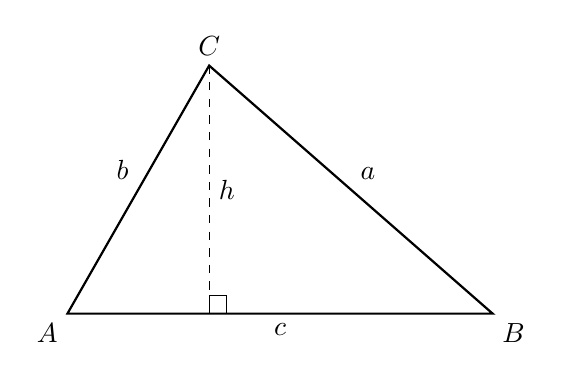
\begin{tikzpicture}[scale=0.9]
\coordinate (A) at (0,0); \coordinate (B) at (6,0); \coordinate (C) at (2,3.5); \coordinate (D) at (2,0);
\draw[thick] (A) -- (B) -- (C) -- cycle;
\draw[dashed] (C) -- (D) node[midway, right] {$h$};
\draw (2,0) -- (2,0.25) -- (2.25,0.25) -- (2.25,0);
\node[below left] at (A) {$A$}; \node[below right] at (B) {$B$}; \node[above] at (C) {$C$};
\node[below] at (3,0) {$c$};
\node[above left] at (1,1.75) {$b$};
\node[above right] at (4,1.75) {$a$};
\end{tikzpicture}
\caption{Side $a$ is opposite angle $A$, and so on. The dashed altitude $h$ splits
the triangle into two right triangles.}
\label{fig:general-triangle}
\end{figure}

\section{The Law of Sines}\index{Law of Sines}

Drop the altitude $h$ from $C$, as in figure \ref{fig:general-triangle}. It splits
the triangle into two right triangles. In the left one, the hypotenuse is $b$, so
$h = b\sin A$. In the right one, the hypotenuse is $a$, so $h = a\sin B$. Both equal
$h$, so $b\sin A = a\sin B$, which rearranges to $\frac{a}{\sin A} = \frac{b}{\sin B}$.
Dropping an altitude from a different corner brings in $c$ the same way.

\begin{mdframed}[style = important, frametitle = {The Law of Sines}]
In any triangle,
$$\frac{a}{\sin A} = \frac{b}{\sin B} = \frac{c}{\sin C}$$
\end{mdframed}

In words: each side is proportional to the sine of the angle across from it.
Bigger angles sit across from longer sides.

Use the Law of Sines when you know an angle and the side across from it, plus one
more piece.

\textbf{Example}: In a triangle, $A = 50^\circ$, $B = 60^\circ$, and $a = 10$. Solve
the triangle.

\textbf{Solution}: The angles add up to $180^\circ$, so $C = 70^\circ$. Then
$$b = \frac{a\sin B}{\sin A} = \frac{10\sin 60^\circ}{\sin 50^\circ} \approx 11.31, \qquad
c = \frac{a\sin C}{\sin A} = \frac{10\sin 70^\circ}{\sin 50^\circ} \approx 12.27$$
Check: the largest angle, $C$, is across from the longest side, $c$.

\subsection{The Ambiguous Case}\index{ambiguous case}
In the Congruence chapter, you learned that there is no SSA test: two sides and an
angle that is not between them do not always pin down a triangle. Here is that
fact in action.

\textbf{Example}: Solve the triangle with $A = 40^\circ$, $a = 7$, and $b = 10$.

\textbf{Solution}: The Law of Sines gives
$$\sin B = \frac{b\sin A}{a} = \frac{10\sin 40^\circ}{7} \approx 0.918$$
The calculator says $B = \sin^{-1}(0.918) \approx 66.7^\circ$. But there is a
second angle with the same sine: $180^\circ - 66.7^\circ = 113.3^\circ$. (The
height of a point on a circle is the same at $\theta$ and at $180^\circ - \theta$,
as you will see in the next chapter.) Both work, because each leaves room for
$C$:
\begin{itemize}
\item $B \approx 66.7^\circ$, $C \approx 73.3^\circ$, $c \approx 10.4$
\item $B \approx 113.3^\circ$, $C \approx 26.7^\circ$, $c \approx 4.9$
\end{itemize}
Two different triangles fit the same three facts. Figure \ref{fig:ambiguous} shows
why: a side of length $a$ swinging from $C$ can reach the bottom line in two
places.

\begin{figure}[H]
\centering
\begin{tikzpicture}[scale=0.75]
\coordinate (A) at (0,0); \coordinate (C) at (6.928,4);
\coordinate (B1) at (3.928,0); \coordinate (B2) at (9.928,0);
\draw[thick] (-0.5,0) -- (11,0);
\draw[thick] (A) -- (C) node[midway, above left] {$b$};
\draw[dashed, gray] (C) ++(-150:5) arc (-150:-30:5);
\draw[thick, sdkblue] (C) -- (B1) node[midway, left] {$a$};
\draw[thick, orange] (C) -- (B2) node[midway, right] {$a$};
\fill (A) circle (2pt) node[below] {$A$};
\fill (C) circle (2pt) node[above] {$C$};
\fill[sdkblue] (B1) circle (2pt) node[below] {$B_1$};
\fill[orange] (B2) circle (2pt) node[below] {$B_2$};
\end{tikzpicture}
\caption{The ambiguous case. With angle $A$ and sides $b$ and $a$ fixed, the side
$a$ can end at $B_1$ or at $B_2$.}
\label{fig:ambiguous}
\end{figure}

If $\frac{b\sin A}{a}$ comes out bigger than 1, there is no triangle at all: side
$a$ is too short to reach. And if the second angle leaves no room
($A + B \geq 180^\circ$), there is only one.

\begin{Exercise}[title={Law of Sines}, label=ls_aas]
In a triangle, $A = 35^\circ$, $C = 105^\circ$, and $c = 20$. Find $B$, $a$, and $b$.
\end{Exercise}
\begin{Answer}[ref=ls_aas]
$B = 180^\circ - 35^\circ - 105^\circ = 40^\circ$. Then
$a = \frac{20\sin 35^\circ}{\sin 105^\circ} \approx 11.88$ and
$b = \frac{20\sin 40^\circ}{\sin 105^\circ} \approx 13.31$.
\end{Answer}

\begin{Exercise}[title={How Many Triangles?}, label=ls_ssa]
How many triangles have $A = 30^\circ$ and $b = 8$, if
\begin{enumerate}
\item $a = 5$?
\item $a = 3$?
\end{enumerate}
\end{Exercise}
\begin{Answer}[ref=ls_ssa]
\begin{enumerate}
\item $\sin B = \frac{8\sin 30^\circ}{5} = 0.8$, so $B \approx 53.1^\circ$ or
$B \approx 126.9^\circ$. Both leave room for $C$ ($30^\circ + 126.9^\circ < 180^\circ$),
so there are two triangles.
\item $\sin B = \frac{8\sin 30^\circ}{3} \approx 1.33$. No angle has a sine greater
than 1, so there is no triangle: side $a$ is too short to reach.
\end{enumerate}
\end{Answer}

\section{The Law of Cosines}\index{Law of Cosines}

The Law of Sines needs an angle and the side across from it. If you know two sides
and the angle \emph{between} them, or all three sides, you need the Law of Cosines.

Put angle $C$ at the origin, with side $b$ along the $x$-axis, so $A$ is at
$(b, 0)$. Side $a$ leaves the origin at angle $C$, so its far end is at
$B = (a\cos C,\ a\sin C)$. (Picture a right triangle with hypotenuse $a$ under that
point.) Side $c$ runs from $A$ to $B$, so by the distance formula,
\begin{align*}
c^2 &= (a\cos C - b)^2 + (a\sin C)^2 \\
    &= a^2\cos^2 C - 2ab\cos C + b^2 + a^2\sin^2 C \\
    &= a^2(\cos^2 C + \sin^2 C) + b^2 - 2ab\cos C \\
    &= a^2 + b^2 - 2ab\cos C
\end{align*}
using the Pythagorean identity in the last step. (This picture assumes $C$ is
acute, but the formula holds for every angle once you meet the cosine of obtuse
angles in the next chapter.)

\begin{mdframed}[style = important, frametitle = {The Law of Cosines}]
In any triangle,
$$c^2 = a^2 + b^2 - 2ab\cos C$$
\end{mdframed}

When $C = 90^\circ$, $\cos C = 0$, and this is the Pythagorean theorem. The
$-2ab\cos C$ term is a correction for angles that are not right: a narrower angle
pulls the ends closer together, and a wider one pushes them apart.

\textbf{Example}: To measure across a pond, a surveyor stands at a point $C$ on
shore. One end of the pond is 120 m away, the other is 150 m away, and the angle
between the two sight lines is $70^\circ$. How wide is the pond?

\textbf{Solution}:
$$c^2 = 120^2 + 150^2 - 2(120)(150)\cos 70^\circ \approx 14400 + 22500 - 12313 = 24587$$
so $c \approx 156.8$ m.

\textbf{Example}: A triangle has sides 5, 6, and 7. Find its largest angle.

\textbf{Solution}: The largest angle is across from the longest side, so let $c = 7$
and solve the Law of Cosines for $\cos C$:
$$\cos C = \frac{a^2 + b^2 - c^2}{2ab} = \frac{25 + 36 - 49}{60} = 0.2
\quad\Longrightarrow\quad C = \cos^{-1}(0.2) \approx 78.5^\circ$$

\subsection{The Area of Any Triangle}\index{triangle!area}
The altitude gives one more useful formula. In figure \ref{fig:general-triangle}, the
area is $\frac{1}{2}(\text{base})(\text{height}) = \frac{1}{2}ch$, and $h = b\sin A$, so
$$\text{Area} = \frac{1}{2}bc\sin A$$
Half the product of two sides times the sine of the angle between them. For example,
a triangle with sides 8 and 11 and a $40^\circ$ angle between them has area
$\frac{1}{2}(8)(11)\sin 40^\circ \approx 28.3$.

\section{Which Tool Should I Use?}
\begin{center}
\begin{tabular}{l|l}
What you know & What to use \\
\hline
A right triangle & SOH-CAH-TOA and the Pythagorean theorem \\
Two angles and any side (AAS or ASA) & Law of Sines \\
Two sides and the angle between them (SAS) & Law of Cosines \\
All three sides (SSS) & Law of Cosines \\
Two sides and an angle not between them (SSA) & Law of Sines, but check for 0, 1, or 2 triangles \\
\end{tabular}
\end{center}

\section{Triangles in Python}
Python's \mintinline{python}{math} library has \mintinline{python}{sin},
\mintinline{python}{cos}, and their inverses, but they work in radians, not degrees.
The functions \mintinline{python}{math.radians} and \mintinline{python}{math.degrees}
convert back and forth:
\begin{minted}{python}
from math import sin, cos, acos, sqrt, radians, degrees

def third_side(a, b, angle_C):
    """Law of Cosines: the side opposite angle C (in degrees)."""
    C = radians(angle_C)          # math.cos expects radians
    return sqrt(a**2 + b**2 - 2*a*b*cos(C))

def angle_opposite(a, b, c):
    """Law of Cosines, solved for the angle opposite side c."""
    return degrees(acos((a**2 + b**2 - c**2) / (2*a*b)))

print(round(third_side(120, 150, 70), 1))   # the pond
print(round(angle_opposite(5, 6, 7), 1))    # the 5-6-7 triangle
print(round(third_side(3, 4, 90), 1))       # a right angle gives Pythagoras
\end{minted}
\begin{verbatim}
156.8
78.5
5.0
\end{verbatim}

\begin{Exercise}[title={Law of Cosines}, label=lc_sas]
\begin{enumerate}
\item Two sides of a triangle are 8 and 11, and the angle between them is $40^\circ$.
Find the third side.
\item A triangle has sides 7, 8, and 9. Find its largest angle.
\end{enumerate}
\end{Exercise}
\begin{Answer}[ref=lc_sas]
\begin{enumerate}
\item $c^2 = 64 + 121 - 176\cos 40^\circ \approx 50.2$, so $c \approx 7.08$.
\item The largest angle is across from 9:
$\cos C = \frac{49 + 64 - 81}{2(7)(8)} = \frac{32}{112} \approx 0.286$, so
$C \approx 73.4^\circ$.
\end{enumerate}
\end{Answer}

\begin{Exercise}[title={Off Course}, label=lc_ship]
A boat sails 20 km due north, then turns $30^\circ$ to the right and sails another
15 km. How far is it from where it started?
\end{Exercise}
\begin{Answer}[ref=lc_ship]
Turning $30^\circ$ off a straight line makes the angle between the two legs, at the
turning point, $180^\circ - 30^\circ = 150^\circ$. Then
$d^2 = 20^2 + 15^2 - 2(20)(15)\cos 150^\circ \approx 625 + 519.6 = 1144.6$, so
$d \approx 33.8$ km. (Without the turn, it would be 35 km away.)
\end{Answer}

\begin{Exercise}[title={A Triangle Solver}, label=lc_python]
Write a Python function \mintinline{python}{area(a, b, angle_C)} that returns the
area of a triangle from two sides and the angle between them, in degrees. Test it on
the triangle with sides 8 and 11 and a $40^\circ$ angle.
\end{Exercise}
\begin{Answer}[ref=lc_python]
\begin{minted}{python}
from math import sin, radians

def area(a, b, angle_C):
    return 0.5 * a * b * sin(radians(angle_C))

print(round(area(8, 11, 40), 1))   # 28.3
\end{minted}
\end{Answer}
